% Configuration

\documentclass[a4paper]{article}

\linespread{1.1}

\usepackage[utf8]{inputenc} 
\usepackage[T1]{fontenc}
\usepackage[francais]{babel}
\usepackage{amsmath}
\usepackage{amsfonts}
\usepackage{graphicx}
\usepackage{lmodern}
\usepackage{microtype}
\usepackage{hyperref}
\usepackage[margin=1.8cm]{geometry}
\usepackage{pgf,tikz}
\usepackage{mathrsfs}
\usetikzlibrary{arrows}


% Structure

\newcounter{c}
\newcounter{d}
\newcounter{r}
\newcounter{e}

\newcommand{\defi}{\subparagraph{D\'efinition \arabic{c}.\arabic{d} :}\stepcounter{d}}
\newcommand{\prop}{\subparagraph{Proposition \arabic{c}.\arabic{r} :}\stepcounter{r}}
\newcommand{\thm}{\subparagraph{Th\'eor\`eme \arabic{c}.\arabic{r} :}\stepcounter{r}}
\newcommand{\demo}{\subparagraph{D\'emonstration}}
\newcommand{\cor}{\subparagraph{Corollaire \arabic{c}.\arabic{r} :}\stepcounter{r}}
\newcommand{\lem}{\subparagraph{Lemme \arabic{c}.\arabic{r} :}\stepcounter{r}}
\newcommand{\rem}{\subparagraph{Remarque :}}
\newcommand{\chapitre}[1]{\stepcounter{c}\setcounter{e}{0}\setcounter{d}{0}\setcounter{r}{0}\noindent\textbf{\Large#1}\\}
\newcommand{\eq}[1]{\stepcounter{e}\begin{equation}#1\tag{\arabic{c}.\arabic{e}}\end{equation}}

% Notations

\newcommand{\Q}{\mathbb{Q}}
\newcommand{\Z}{\mathbb{Z}}
\newcommand{\N}{\mathbb{N}}
\newcommand{\R}{\mathbb{R}}
\newcommand{\C}{\mathbb{C}}
\newcommand{\E}[1]{\mathbb E\left(#1\right)}
\newcommand{\sph}{\mathbb{S}}
\newcommand{\p}{{\cal{P}}}
\newcommand{\fsp}{{\cal{F}}}
\newcommand*{\qed}{\hfill\ensuremath{\square}}
\newcommand{\x}{\mathbf x}
\newcommand{\y}{\mathbf y}
\newcommand{\e}{\mathbf e}
\newcommand{\scal}[2]{\langle#1,#2\rangle}
\newcommand{\trans}{^\text{T}\!}

\newcommand{\nor}[2]{{\cal N}(#1,#2)}
\newcommand{\mat}[2]{{\cal M}_{#1\times#2}(\R)}

\newcommand{\X}{\mathbf X}

\date{}
\author{Philippe Ricka}
\title{}

\newcommand{\saut}{\vspace{0.5em}}

\begin{document}

%\maketitle

\chapitre{Filtre de Kalman discret (KF)}

On considère un système dynamique stochastique linéaire

\eq{\left\{\begin{array}{l}x_{k+1}=A_kx_k+w_k\\y_k=H_kx_k+v_k\end{array}\right.}

Où
\begin{itemize}
\item $\x_k\in\R^n$ désigne l'état du système
\item $A_k\in\mat nn$ désigne la matrice de transition relative à la dynamique réelle
\item $\y_k\in\R^m$ désigne les mesures relatives à l'état réel $\x$
\item $H_k\in\mat mn$ désigne la matrice de mesure
\item $v_k\in\R^m$ désigne l'erreur d'obervation, qu'on suppose $\nor 0{R_k}$
\item $w_k\in\R^n$ désigne la perturbation du système, qu'on suppose $\nor 0{Q_k}$
\end{itemize}
On suppose de plus que $v_k$ et $w_k$ sont indépendantes.


On mettra en exposant un $f$ (\emph{forecast}) pour les prévisions et un $a$ (\emph{analysis}) pour les analyses.

\saut

On postule l'absence d'erreur du modèle pour la prédiction à partir d'une analyse.

$$\x^f_{k+1}=A_k\x^a_k$$

Une estimation de l'état du système à un instant $t_k$ (analyse) est supposément une combinaison linéaire de la prédiction actuelle et des mesures actuelles.

$$\x^a_k=\tilde L_k\x^f_k+\tilde K_k\y_k\text{ où $\tilde L_k\in\mat nn$ et $\tilde K_k\in\mat nm$ sont des matrices à préciser}$$

On définit formellement les erreurs de prédiction et d'analyse.

$$\begin{array}{lr}\e^f_k=\x^f_k-\x_k&\e^a_k=\x^a_k-\x_k\end{array}$$

où $\x_k$ désigne l'état réel du système.

\prop Si $\tilde L_k=I-\tilde K_kH_k$ et si $\E{\e^f_k}=0$, alors $\E{\e^a_k}=0$.
\demo $$\begin{array}{rl}
\E{\e^a_k}=&\E{\x^a_k}-\x_k\\
=&\E{\tilde L_k\x^f_k+\tilde K_k\y_k}-\x_k\\
=&\E{(I-\tilde K_kH_k)\x^f_k+\tilde K_k\y_k}-\x_k\\
=&\E{\x^f_k-\tilde K_kH_k\x^f_k+\tilde K_k(H_k\x_k+v_k)}-\x_k\\
=&\E{(I-\tilde K_kH_k)\e^f_k}\\
=&0
\end{array}$$\qed

\defi On appelle $\tilde K_k$ la \emph{matrice de gain}. Elle décrit les poids attribués aux observations $\y_k$ et aux mesures $H_k\x^f_k$.

On définit les covariances des erreurs de prévision et d'analyse.

\eq{\begin{array}{lr}P^f_k=\E{\e^f_k\cdot\trans\e^{f}_k}&P^a_k=\E{\e^a_k\cdot^\text{T}\e^{a}_k}\end{array}}

\prop Sous les hypothèses de la proposition précédente, on a :

\eq{\begin{array}{rl}
P^a_k=&(I-\tilde K_kH_k)\cdot P^f_k\cdot\trans(I-\tilde K_kH_k)+\tilde K_k\cdot R_k\cdot\trans\tilde K_k\\
&\\
P^f_k=&A_k\cdot P^a_k\cdot\trans A_k-Q_k
\end{array}}
\demo On pose $Cov(\x)=\E{\x\cdot\trans\x}$.
$$\begin{array}{rl}
P^a_k=&\E{\e^a_k\cdot\trans\e^a_k}=Cov(\e^a_k)\\
=&Cov\left(\tilde L_k\x^f_k+\tilde K_k\y_k-\x_k\right)\\
=&Cov\left((I-\tilde K_kH_k)\x^f_k+\tilde K_k\y_k-\x_k\right)\\
=&Cov\left((I-\tilde K_kH_k)\x^f_k+\tilde K_k(H_k\x_k+v_k)-\x_k\right)\\
=&(I-\tilde K_kH_k)\cdot Cov\left(\x^f_k-\x_k\right)\cdot\trans(I-\tilde K_kH_k)+Cov\left(\tilde K_kv_k\right)\\
=&(I-\tilde K_kH_k)\cdot P_k^f\cdot\trans(I-\tilde K_kH_k)+\tilde K_k\cdot R_k\cdot\trans\tilde K_k\\
&\\
P^f_{k+1}=&Cov\left(\e_{k+1}^f\right)\\
=&Cov\left(\x^f_{k+1}-\x_{k+1}\right)\\
=&Cov\left(A_k\x^a_k-A_k\x_k-w_k\right)\\
=&A_k\cdot Cov(e_k^a)\cdot\trans A_k-Cov\left(w_k\right)\\
=&A_k\cdot P_k^a\cdot\trans A_k-Q_k
\end{array}$$\qed

\rem Dans un modèle parfait, on aurait $Q_k=0$.

\saut

On contruit maintenant ${\mathcal I}_k^a$, un estimateur de la fiabilité des analyses, en mesurant l'écart entre l'analyse et le véritable état. Soit $B_k\in\mat nn$ déterministe diagonale définie positive : la matrice d'échelle. On pose :

\eq{{\cal I}_k^a=\E{\trans\e^a_k\cdot B_k\cdot\e^a_k}=\E{\sum_{i=1}^n(\e^a_k)_im_{ii}(\e^a_k)_i}=\text{Tr}(B_kP^a_k)}

On souhaite minimiser ${\cal I}_k^a$. Cela revient à minimiser $P^a_k$. On va différencier l'application $\varphi:\mat nn\to\R,\tilde K_k\mapsto P^a_k$.
$$\begin{array}{rl}\varphi(\tilde K_k+h)=&(I-(\tilde K_k+h)H_k)\cdot P_k^f\cdot\trans(I-(\tilde K_k+h)H_k)+(\tilde K_k+h)\cdot R_k\cdot\trans(\tilde K_k+h)\\
=&P^f_k-\tilde K_k\cdot H_k\cdot P^f_k-P_k^f\cdot\trans H_k\cdot\trans\tilde K_k+\tilde K_k\cdot H_k\cdot P^f_k\cdot\trans H_k\trans\tilde K_k+\tilde K_k\cdot R_k\cdot\trans\tilde K_k\\
&-h\cdot H_k\cdot P^f_k-P^f_k\cdot\trans H_k\cdot\trans h+h\cdot H_k\cdot P^f_k\cdot\trans H_k\cdot\trans\tilde K_k\\
&+\tilde K_k\cdot H_k\cdot P^f_k\cdot\trans H_k\cdot\trans h+h\cdot R_k\cdot\trans\tilde K_k+\tilde K_k\cdot R_k\cdot\trans h\\
&+h\cdot H_k\cdot P^f_k\cdot\trans H_k\cdot\trans h+h\cdot R_k\cdot\trans h
\end{array}$$

d'où

$$d(\varphi)(\tilde K_k)(h)=-h\cdot (H_k\cdot P^f_k\cdot (I-\trans H_k\cdot \trans\tilde K_k)-R_k\cdot \trans\tilde K_k)-((I-\tilde K_k\cdot  H_k)P^f_k\cdot \trans H_k-\tilde K_k\cdot R_k)\cdot \trans h$$

On cherche $\tilde K_k$ optimale, c'est à dire telle que $d(\varphi)(\tilde K_k)=0$. C'est le cas lorsque :

$$H_k\cdot\trans P^f_k\cdot(I-\trans H_k\cdot\trans\tilde K_k)-\trans R_k\cdot\trans\tilde K_k=0$$

donc lorsque :

\eq{\tilde K_k=P^f_k\cdot\trans H_k\cdot\left(H_k\cdot P^f_k\cdot\trans H_k+R_k\right)^{-1}:=K_k.}

Cette matrice $K_k\in\mat nm$ est appelée le \emph{gain de Kalman}. En l'injectant dans l'expression de $P^a_k$, on trouve

$$\begin{array}{rl}
P^a_k=&(I-K_k\cdot H_k)\cdot P^f_k\cdot\trans(I-K_k\cdot H_k)+K_k\cdot R_k\cdot\trans K_k\\
=&P^f_k-P^f_k\cdot\trans H_k\cdot(H_k\cdot P^f_k\cdot\trans H_k+R_k)^{-1}\cdot H_k\cdot P^f_k\\
&-P^f_k\cdot\trans H_k\cdot(H_k\cdot\trans P^f_k\cdot\trans H_k+\trans R_k)^{-1}\cdot H_k\cdot\trans P^f_k\\
&+P^f_k\cdot\trans H_k\cdot(H_k\cdot\trans P^f_k\cdot\trans H_k+\trans R_k)^{-1}\cdot H_k\cdot\trans P^f_k\\
=&P^f_k\cdot(I-\trans H_k\cdot\trans K_k)\\
=&(I-H_k\cdot K_k)\cdot P^f_k
\end{array}$$

La dernière égalité ayant lieu grâce au caractère symétrique de $P^f_k$.

\newpage
On aboutit finalement à la relation :

\eq{\x^a_k=\x^f_k+K_k(\y_k-H_k\x^f_k).}

La procédure s'itère dans le temps suivant les étapes :

\saut

\begin{tabular}{p{3cm}|l}
Analyse &$K_k = P^f_k\cdot H_k\cdot(H_k\cdot P^f_k\cdot \trans H_k + R_k)^{-1}$\\
&$\x^a_k = \x^f_k + K_k\cdot(\y_k - H_k\cdot\x^f_k)$\\
&$P^a_k = (I-K_k\cdot H_k)\cdot P^f_k$\\
\end{tabular}

\saut

\begin{tabular}{p{3cm}|l}
Prédiction &$\x^f_{k+1} = A_k\cdot \x^a_k$\\
&$P^f_{k+1} = A_k\cdot P^a_k\cdot\trans A_k +Q_k$
\end{tabular}


\bigskip
\chapitre{Exemple : chute d'un mobile}

On considère la chute d'un mobile soumis à une accélération de la pesanteur $g$ au cours d'un intervalle de temps $[0,T]$ discrétisé avec un pas $dt$. On note sa position, sa vitesse et son accélération au temps $k.dt$ respectivement $x_k$, $x'_k$ et $x''_k$. Le vecteur d'état du système à un instant $k.dt$ est :

$$\x_k=\left(\begin{matrix}x_k\\x'_k\\x''_k\end{matrix}\right).$$

La physique nous renseigne sur la matrice de transition $A$ d'un instant au suivant :

$$A=\left(\begin{matrix}1&dt&dt^2\\0&1&dt\\0&0&1\end{matrix}\right)$$

de façon à ce que la relation de récurrence suivante ait lieu :

$$\x_{k+1}=A\cdot\x_k+\mathbf w_k$$

où $\mathbf w_k\sim\mathcal{N}(0,Q)$ pour une matrice de covariance $Q$ fixée. En supposant que les bruits affectant la position, la vitesse et l'accélération sont indépendants, on trouve :

$$Q=\left(\begin{matrix}(w_k)^2&0&0\\0&(w_k')^2&0\\0&0&(w_k'')^2\end{matrix}\right).$$

On relève à chaque instant l'état du système en commettant une erreur $\mathbf v_k$ :

$$\y_k=H\cdot\x_k+\mathbf v_k=\x_k+\mathbf v_k$$

en prenant $H=I_3$, où $\mathbf v_k\sim\mathcal N(0,R)$ pour une matrice de covariance diagonale fixée $R$ (on suppose les erreurs de mesure indépendantes).

\saut

En considérant le pas de temps $dt$ suffisamment petit, il est raisonnable d'initialiser \verb Pf= $P^f_1=R$.

Les matrices impliquées dans nos calculs ont des expressions relativement simples grâce à l'hypothèse $H=I_3$, qui revient à supposer que l'on mesure directement les grandeurs qui nous intéressent.

\newpage
\begin{verbatim}

génération des états réels x_k bruités par w_k de covariance Q
génération des mesures y_k bruitées par v_k de covariance R

Pf = R ;
xf(1) = y(1);

pour k de 2 à T/dt
    K = Pf * inv(Pf + R);
    xa = xf(:,i-1) + K * (y(:,i) - xf(:,i-1));
    Pa = (I - K) * Pf;
  
    xf(:,i) = A * xa;
    Pf = A * Pa * A' + Q;
fin

\end{verbatim}


La figure 1 illustre les résultats obtenus pour la position et la vitesse d'un mobile dans le cas où :
\begin{itemize}
\item $g=-9.81 m.s^{-2}$,
\item $dt=0.2 s$,
\item $T=5 s$,
\item $\x_1=\trans\left(\begin{matrix}0&0&0\end{matrix}\right)$,
\item $w_k=1$, $w_k'=0.5$, $w_k''=0.25$,
\item $v_k=5$, $v_k'=5$, $v_k''=10$.
\end{itemize}




\begin{figure}[!h]
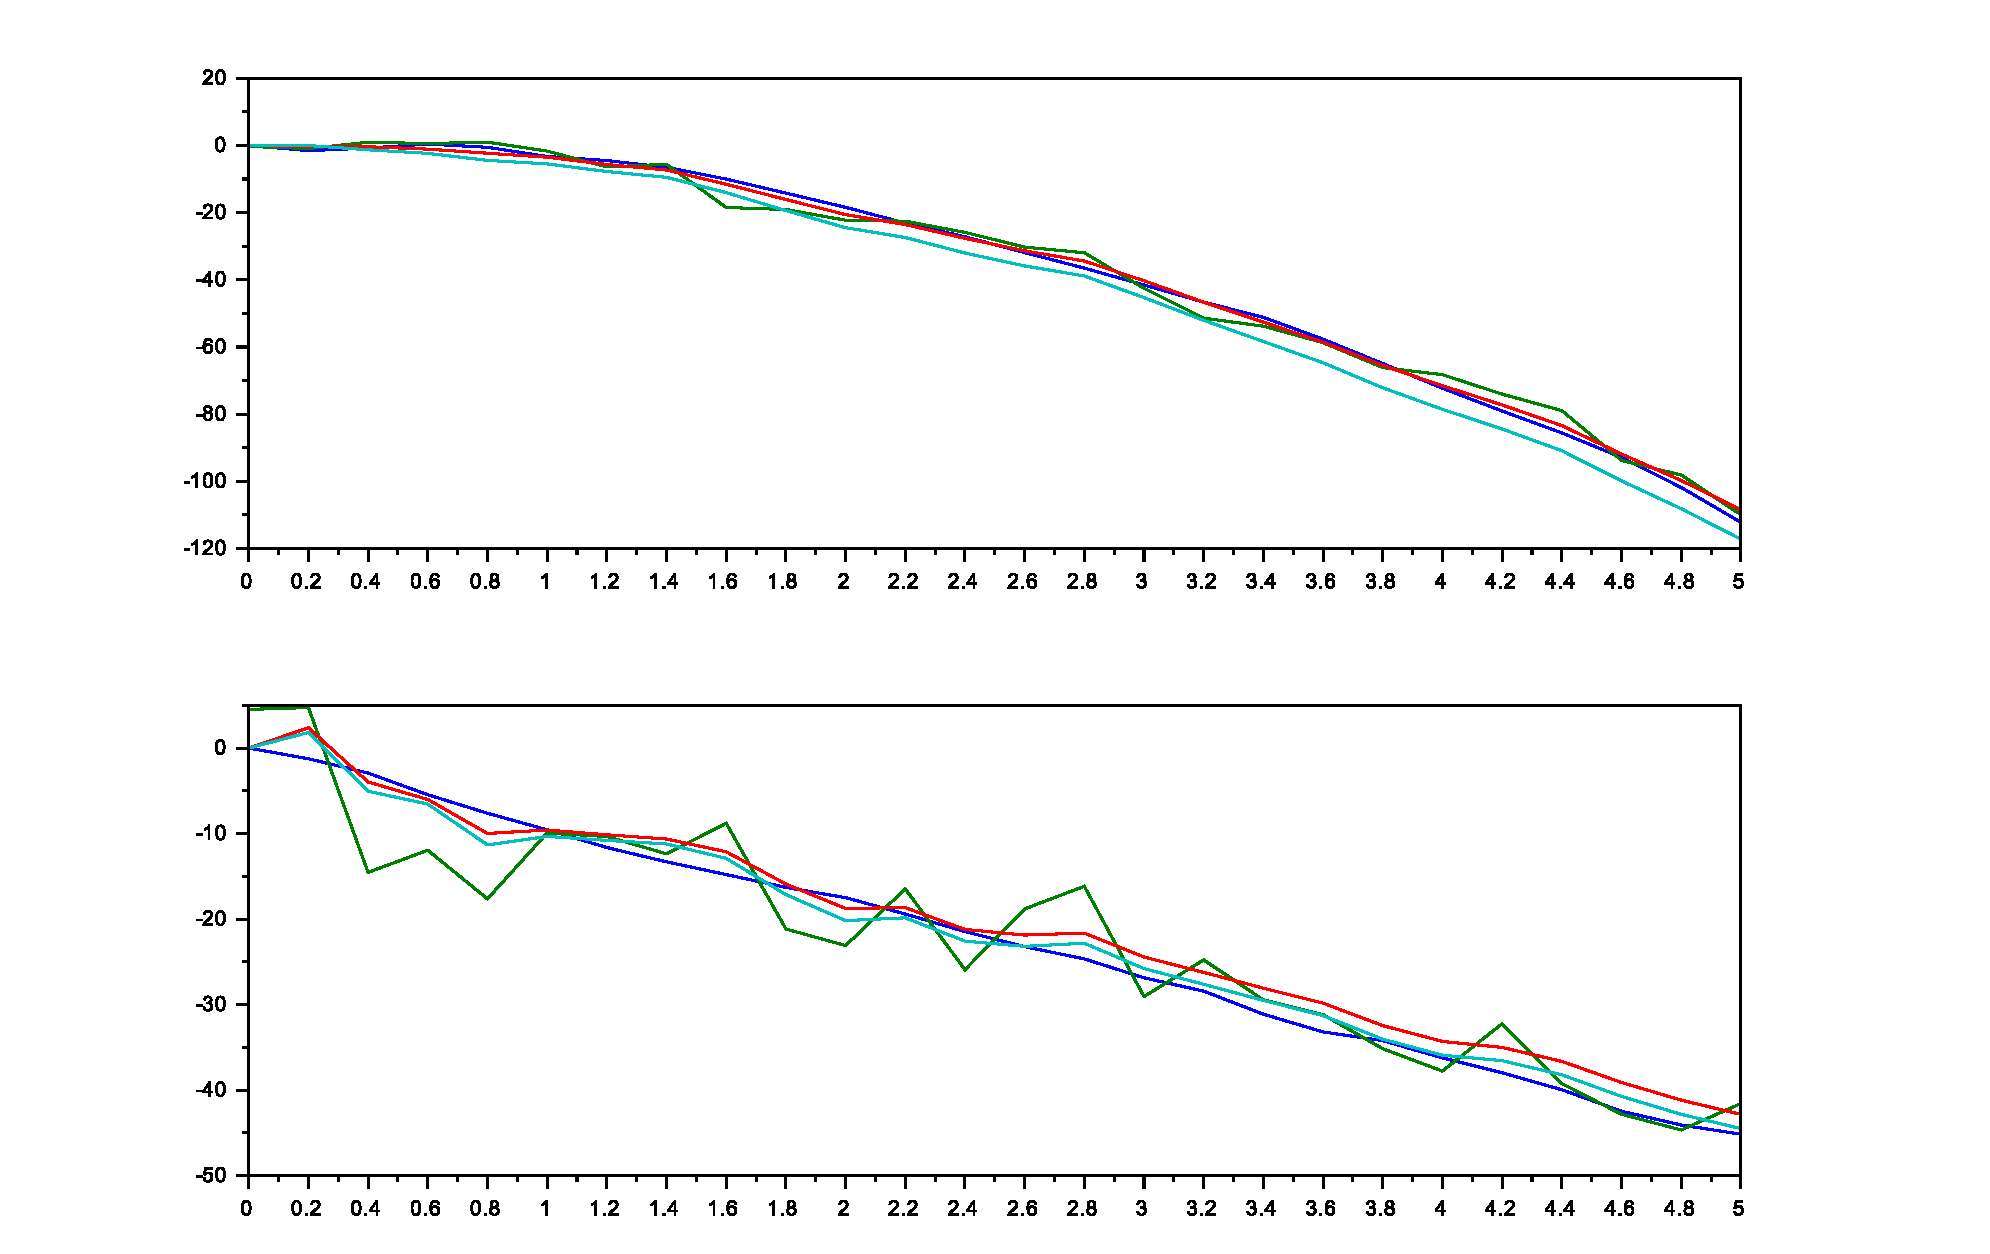
\includegraphics[width=\textwidth]{KalmanMobile.pdf}
\caption{En bleu : $\x$. ; en vert : $\y$ ; en rouge : $\x^a$ ; en cyan : $\x^f$.}
\end{figure}


\newpage
\chapitre{Filtre de Kalman à ensemble (EnKF) - dynamique explicite}

Ce filtre fonctionne sur le meme principe que le KF, à ceci près qu'on évalue $P^f_k$ à partir d'un ensemble $\{\x^{fi}_k|i=1,...,q_{ens}\}$ où $q_{ens}>1$ est un entier. Dans le cas où la dynamique du système est décrite par une fonction linéaire ou par une fonction très régulière, on préfèrera le KF appliqué à cette fonction ou à la fonction linéarisée pour des raisons de coût. En revanche, l'EnKF dévoile ses performances dans le cas des processus non-linéaires. En toute généralité :

\eq{\left\{\begin{array}{l}\x_{k+1} = f(\x_k,\mathbf u_k)+\mathbf w_k\\\y_k=h(\x_k)+\mathbf v_k\end{array}\right.}

où les notations employées sont les mêmes que précédemment, et $f$ désigne la fonction décrivant la dynamique du système et $\mathbf u_k$ est un paramètre du système.



Au premier pas, on se munit d'un ensemble d'estimations initiales $\X_1 = \{\x^{fi}_1|i=1,...,q_{ens}\}$, et on suppose à chaque pas qu'on dispose d'une telle famille $\X_k$. On définit la prédiction moyenne :

\eq{\overline{\x_k^f}=\frac1{q_{ens}}\sum_{i=1}^{q_{ens}}\x_k^{fi}.}

La matrice de covariance de l'erreur de prédiction est alors :

\eq{P^f_k=\frac1{q_{ens}-1}\sum_{i=1}^{q_{ens}}(\x_k^{fi}-\overline{\x_k^f})\cdot\trans(\x_k^{fi}-\overline{\x_k^f}).}


On bruite $q_{ens}$ fois la mesure de façon à produire une famille $\{\y_k^i=\y_k+\mathbf e_k^i|i=1,...,q_{ens}\}$ où chaque $\mathbf e_k^i$ est gaussien de taille $m$ et de faible variance.


Pour calculer le gain de Kalman, il est nécessaire de construire la matrice $R_k$. Par indépendance des bruits, elle doit être diagonale. On trouve dans la littérature :

\eq{R_k = \text{diag}\left(\frac1{q_{ens}-1}E\cdot\trans E\right)}

où $E=(\mathbf e_k^1,...,\mathbf e_k^{q_{ens}})\in\mat m{q_{ens}}.$

Le gain de Kalman s'exprime de la même façon que dans le cas précédent ; toutefois, $H_k$ désigne l'approximation linéaire de $h$ au voisinage de $\x_k$, ce qui peut être délicat à calculer. D'après Houtekamer et Mitchell si $\overline{h(\x_k^f)}=h(\overline{\x_k^f})$ et si $\|\x_k^{fi}-\overline{\x_k^f}\|$ est assez petit pour tout $i$, alors les approximations suivantes sont raisonnables :

\eq{P^f_{\x\y_k}=P^f_k\cdot\trans H_k\simeq\frac1{q_{ens}-1}\sum_{i=1}^{q_{ens}}(\x_k^{fi}-\overline{\x_k^f})\cdot\trans(h(\x_k^{fi})-h(\overline{\x_k^f}))}

\eq{P^f_{\y\y_k}=H\cdot P^f_k\cdot\trans H+R_k\simeq\frac1{q_{ens}-1}\sum_{i=1}^{q_{ens}}(h(\x_k^{fi})-\overline{h(\x_k^f)})\cdot\trans(h(\x_k^{fi})-\overline{h(\x_k^f)})+R_k.}



Il suffit alors de remarquer que :

\eq{K_k = P^f_{xy_k}\cdot\left(P^f_{yy_k}\right)^{-1}.}


En somme, on applique l'algorithme suivant :

\begin{verbatim}
pour k de 2 à T/dt
    pour i de 1 à qens
        xf(i) = f(xa(i),uk) + w(i);
    fin
    Pxy = formule (3.5);
    Pyy = formule (3.6);
    K = Pxy*inv(Pyy);
    pour i de 1 à qens
        y(i) = yk + e(i);
        xa(i) = xf(i) + K*(y(i) -  h(xf(i)))
    fin
fin
\end{verbatim}

\chapitre{Filtre de Kalman à ensemble - dynamique implicite}

Il arrive souvent que l'utilisateur n'ait pas accès directement à la fonction $f$ relative à la dynamique du système. Dans ce cas, on peut se contenter d'admettre que $x^f$ suit une marche aléatoire :

\eq{x^f_{k+1}=x^f_k+\delta_k}

où $\delta_k\sim\nor0{D_k}$. En reprenant l'exemple précédent, on condsidère que la marche aléatoire concerne indépendamment chaque composante de $\x$. La matrice $D_k$ est alors diagonale. Dans le but d'approcher la dynamique réelle, choisissons :

$$D_k(1,1)=(x_k-x_{k-1})^2=(x'_0dt+g(2k-1)dt^2)^2$$
$$D_k(2,2)=(x'_k-x'_{k-1})^2=(gdt)^2$$

La matrice $D_k$ devant être définie positive, on choisit un $\varepsilon>0$ très petit et on pose :

$$D_k(3,3)=\varepsilon.$$

Dans l'exemple, nous avons arbitrairement pris $\varepsilon=dt$.


\begin{figure}[!h]
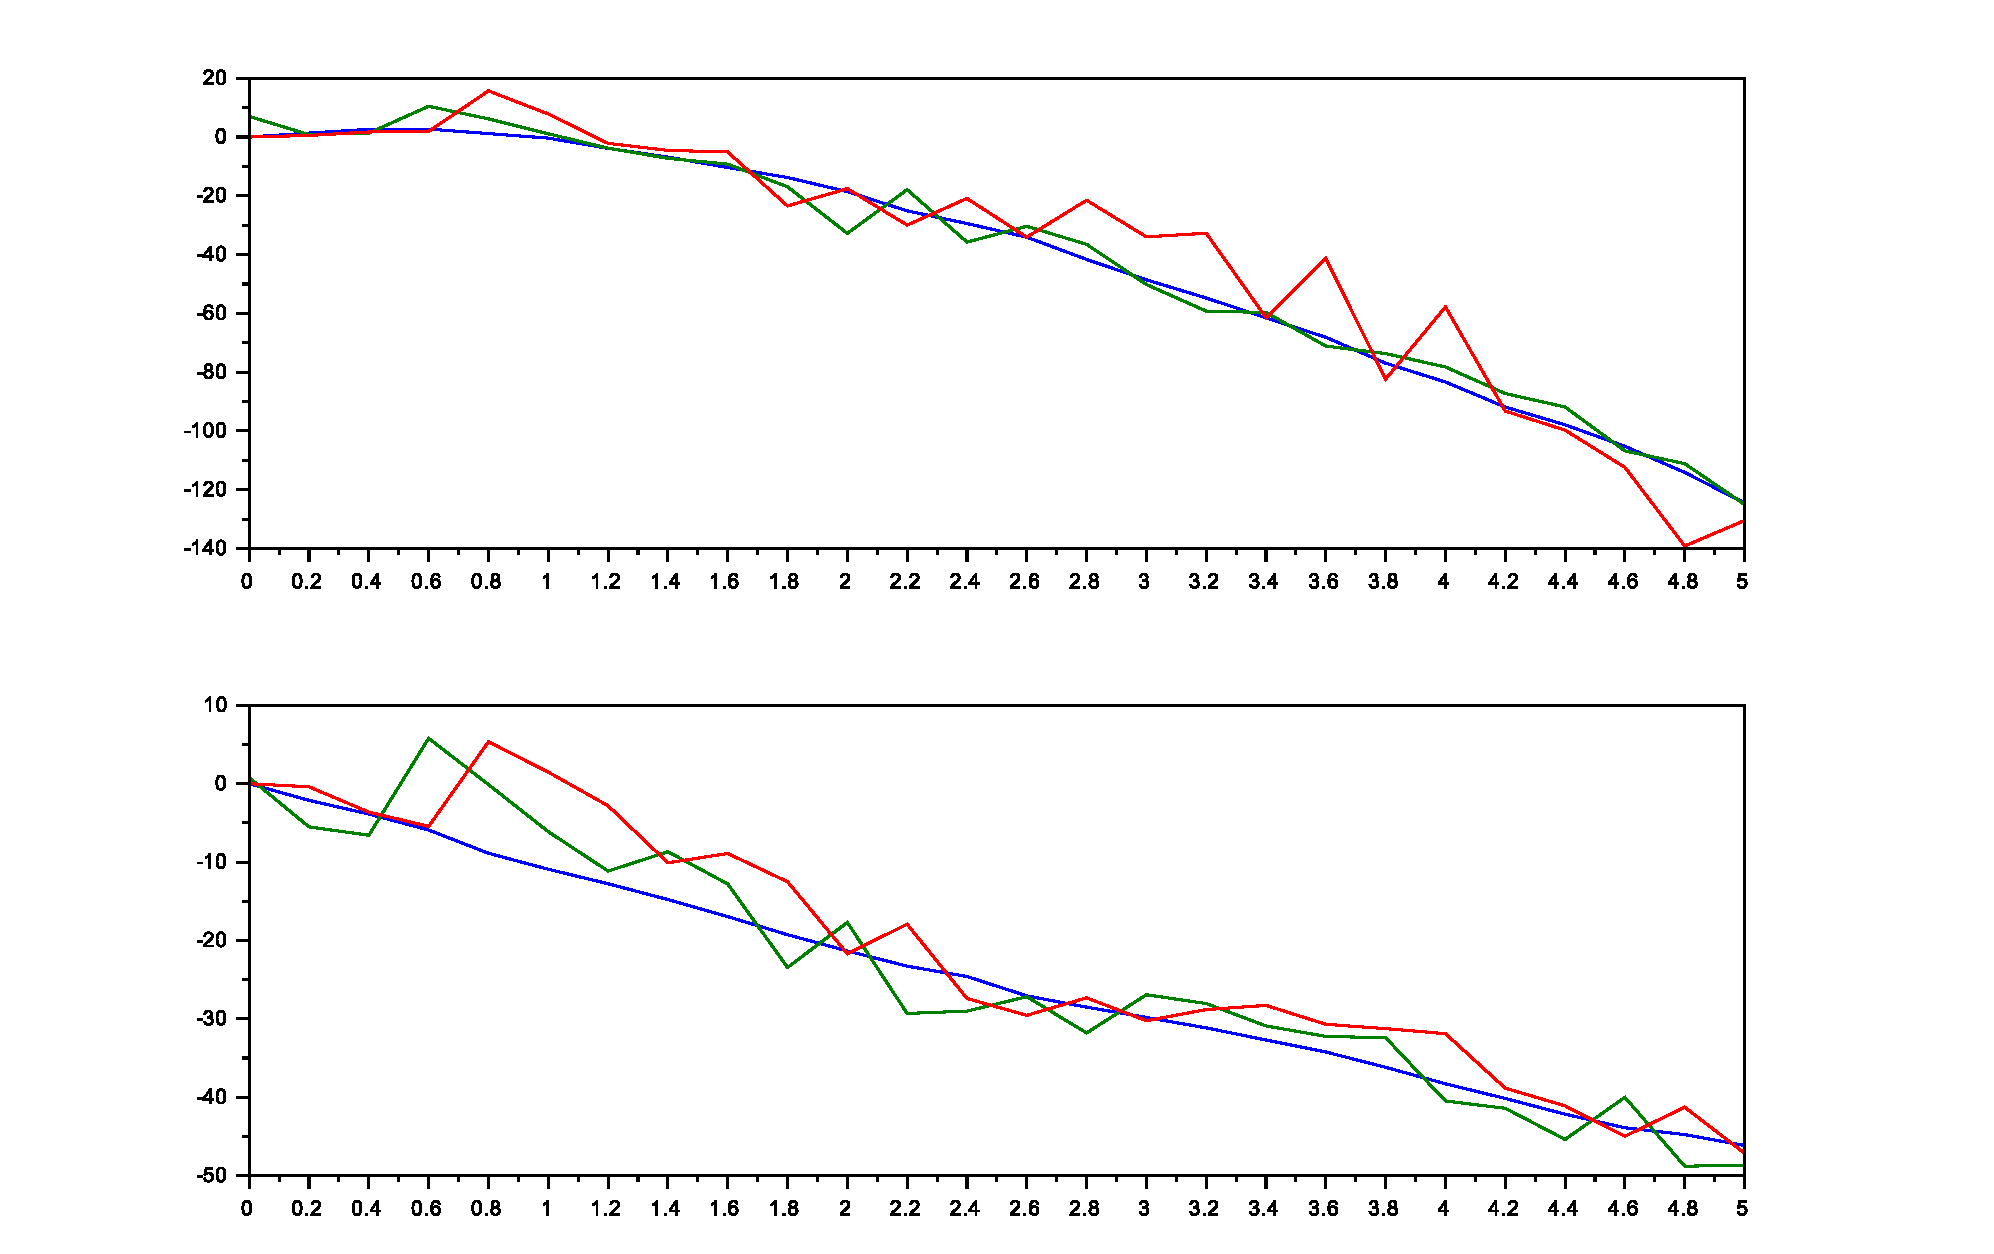
\includegraphics[width=\textwidth]{ENKalmanMobile.pdf}
\caption{En bleu : $\x$ ; en vert : $\y$ ; en rouge : $\overline{\x^f}$.}
\end{figure}

L'algorithme devient :

\begin{verbatim}
pour k de 2 à T/dt
    Dk = diag( (y1(2)*dt + g*(2*k-1)*dt)^2 , (g*dt)^2 , dt);
    pour i de 1 à qens
        xf(i) = xa(i) + delta;
        yk(i) = yk + e;
    fin
    Pxy = formule (3.5);
    R = formule (3.4);
    Pyy = formule (3.6);
    K = Pxy*inv(Pyy);
    pour i de 1 à qens
        xa(i) = xf(i) + K*(y(i) - h(xf(i)));
    fin
fin

\end{verbatim}


On voit que la fonction dynamique $f$ n'intervient à aucun moment. La prédiction est évidemment moins précise que dans le cas discret, mais cette méthode permet de produire une prédiction à propos d'un système dont on ne connait \emph{a priori} pas la dynamique. Sur le même exemple que précédemment, on obtient les résultats représentés dans la figure 2.


Ce type de filtre de Kalman permet en particulier d'estimer les paramètres d'un système. Dans sa thèse, R. Lal obtient d'excellentes estimations de la viscosité, de la vitesse d'advection et des conditions initiales dans le cadre de l'équation d'advection-diffusion avec $q_ens = 4$, $T=100$, $dt=0,15$, à partir d'une simulation \emph{in silico}.

\saut
\saut
\chapitre{Bibliographie}

[Lal17] R. Lal \emph{Data assimilation and uncertainty quantification in cardiovascular biomechanics}, thèse (2017)


[TC94] R. Todling, S.C. Cohn \emph{Suboptimal schemes for atmospheric data assimilation based on the Kalman filter}, Data Assimilation Office, NASA/Goddard Space Flight Center, Greenbelt, Maryland (1994)







\end{document}
